Support vector machines (SVM) can be used for forecasting in the commodity market. In \cite{xie2006new} they use SVMs for predicting the crude oil prices. SVMs are by nature a linear learning machine which means SVMs always use linear functions to solve the regression analysis. However they can be expanded to be able to solve nonlinear problems. This is done by mapping the data into a high-dimensional feature space using a nonlinear mapping. Afterwards it is possible to use linear regression on this space to solve nonlinear problems. The SVMs undergo four different phases before being able to make predictions. These can be seen in figure ~\ref{fig:phasesOfSVM}
\begin{figure}[weight!]
\centering
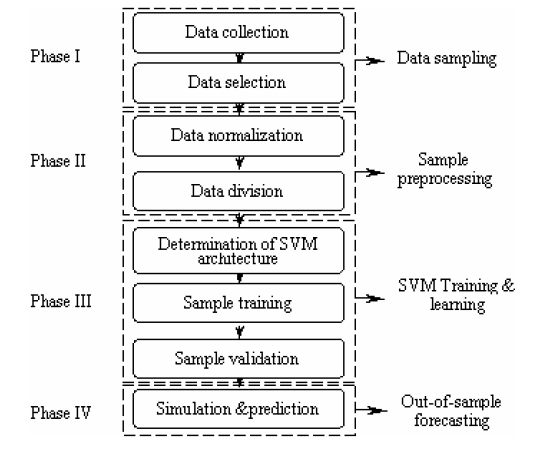
\includegraphics[width=0.8\textwidth ,natwidth=410,natheight=237]{billeder/phases_of_SVM.png}
\caption{The steps taken to create a Support Vector Machine}
\label{fig:phasesOfSVM}
\end{figure}
Data sampling is done daily but due to inconsistencies in these data they adopt weekly and monthly data as alternatives. Data preprocessing is done by transforming the data into more appropriate data for learning purposes. This can be done by using logarithmic transformation or other data transformations. The training and learning step is used for determining the architecture and the parameters of the SVM. There is no criterion for deciding these other than just trial-and-error and the developers experience in the field. Out-of-sample forecasting is done on new data and the prediction is made. As for evaluation they use the Root Mean Square Error (RMSE) to describe the estimated deviation from the real values. Their results and analysis shows that their SVM performs better than both ARIMA and Back Propagation Neural Networks. They argue that SVMs gives better predictions than ARIMA and BPNNs in most cases but neural networks might perform better with data that is optimized for neural networks. Also the neural network outperforms the SVM in one of their sub-period comparisons.

SVMs have also been used for load forecasting of electricity demand. In \cite{chen2004load} they use SVMs to make short-term predictions such as one-day ahead predictions. The goal of this study was to win a competition held by the EUNITE (EUropean Network on Intelligent TEchnologies for Smart Adaptive Systems). This was the winning proposal in the competition. They first examined the data which was half-hourly load demands which had been recorded from 1997 to 1998. In the pursuit of winning the competition they analyzed the data and figured out that in the wintertime load demand was higher than in the summertime thus indicating a connection to weather data and a separation of data was possible. The weekends could also be separated from the weekdays since the weekend load was lower than regular weekdays. When analysis was done they started setting up the model. First of all they prepared the data and selected the data needed for the prediction. They selected calendar attributes to map the holidays and which day it was to account for lower demands. Temperature was included in the vectors used for prediction of the electricity load demand and historical data was incorporated as well. The data segmentation in the steps of preparing a SVM allowed them to take only a subset of the data since most of it could be generalized in the data analysis thus making it easier to do computations. They argue that their model for forecasting demand loads were the best possible model used in this competition and to give a more varied view on this they try out other methods; among these Neural Networks. They configured a neural network that first performed work on the same data as their Support Vector Machine and it provided less than satisfactory feedback with an error margin of 6-8\%. If they took the basic values used in the competition without doing any precomputation on it they received a much better result of 3.64\%. From this they conclude that their SVM performed better than Neural Networks in the specific problem and that neural networks performance depends heavily on the data used as input. 